\documentclass[ngerman,hyperref={pdfpagelabels=false}]{beamer}

% -----------------------------------------------------------------------------

\graphicspath{{images/}}

% -----------------------------------------------------------------------------

\usetheme{KIT}

\setbeamercovered{transparent}
%\setbeamertemplate{enumerate items}[ball]

\newenvironment<>{KITtestblock}[2][]
{\begin{KITcolblock}<#1>{#2}{KITblack15}{KITblack50}}
{\end{KITcolblock}}

\usepackage[ngerman,english]{babel}
\usepackage[utf8]{inputenc}
\usepackage[TS1,T1]{fontenc}
\usepackage{array}
\usepackage{multicol}
\usepackage[absolute,overlay]{textpos}
\usepackage{beamerKITdefs}
\usepackage{algorithm,algpseudocode}

\pdfpageattr {/Group << /S /Transparency /I true /CS /DeviceRGB>>}	%required to prevent color shifting withd transparent images


\title{Algorithmen I - Tutorium 5}
\subtitle{Sebastian Schmidt -- \textit{isibboi@gmail.com}}

\author[Sebastian Schmidt]{Sebastian Schmidt}
\institute{Arbeitsgruppe Kryptographie und Sicherheit}

\TitleImage[width=\titleimagewd,height=\titleimageht]{titel}

\KITinstitute{Arbeitsgruppe Kryptographie und Sicherheit}
\KITfaculty{Fakult\"at f\"ur Informatik}

\newcommand{\encode}[2]{\only<1>{#1}\only<2->{#2}}


% -----------------------------------------------------------------------------

\begin{document}
\setlength\textheight{7cm} %required for correct vertical alignment, if [t] is not used as documentclass parameter


% title frame
\begin{frame}
  \maketitle
\end{frame}

\begin{frame}{Sortieren}
\begin{itemize}[<+->]
\item Eines der verbreitetsten Probleme der Informatik
\item In jeder Sprache in der Standardbibliothek vorhanden
\item Wichtig für schnelle Indexdatenstrukturen jeder Art
\item Quicksort beliebtes Thema von Bewerbungsgesprächen
\item Easy to learn - Hard to master
\end{itemize}
\end{frame}

\begin{frame}{Das Problem}
Gegeben eine Folge von $n$ Elementen $\alpha_1, ..., \alpha_n$.

Finde eine Permutation $\sigma$, sodass gilt:

$\forall i \in \{1, \dots, n - 1\} : \alpha_{\sigma(i)} \leq \alpha_{\sigma(i + 1)}$
\end{frame}

\begin{frame}{Die Lösungen}
\begin{multicols}{2}
\begin{itemize}
\footnotesize
\item Binary Tree Sort (höhen-balanciert)
\item Binary Tree Sort
\item Bogosort
\item Bubblesort
\item Bucketsort
\item Combsort
\item Countingsort
\item Flashsort
\item Gnomesort
\item Heapsort
\item \only<3>{\color{red}}Insertionsort\only<3>{\color{black}}
\item Introsort
\item Merge Insertion
\item \only<3>{\color{red}}Mergesort\only<3>{\color{black}}
\item Natural Mergesort
\item Quicksort
\item Radixsort (LSB)
\item Radixsort (MSB)
\item \only<3>{\color{red}}Selectionsort\only<3>{\color{black}}
\item Shakersort (Cocktailsort)
\item Shellsort
\item Slowsort
\item Smoothsort
\item Stoogesort
\item Swap-Sort
\item Timsort
\end{itemize}
\end{multicols}

\pause

$\Rightarrow$ Es machen sich sehr viele Leute sehr viele Gedanken darüber, wie man schnell sortiert.
\end{frame}

\begin{frame}{Ein Sortieralgorithmus}
\only<1-2>{Wie heißt der Algorithmus?}

\only<3>{Welche Laufzeit hat der Algorithmus im Worst-Case im $O$-Kalkül?
Was ist eine Worst-Case-Eingabe?}

\only<4>{Welche Laufzeit hat der Algorithmus im Best-Case im $O$-Kalkül?
Was ist eine Best-Case-Eingabe?}

\only<5>{Welche Laufzeit hat der Algorithmus im Average-Case im $O$-Kalkül?}

\only<6>{Wie ist der zusätzliche Speicherbedarf im $O$-Kalkül?}

\only<7>{Ist der Sortieralgorithmus stabil?}

\begin{algorithm}[H]
\begin{algorithmic}
\Function{\encode{Sort}{SelectionSort}}{$A : Number[1, \dots, n$]}
\For{$\encode{i}{sorted}$ from $1$ to $n - 1$}
\State $\encode{k}{minIndex} \gets \encode{i}{sorted}$
\For{$\encode{j}{index}$ from $\encode{i}{sorted} + 1$ to $n$}
\If{$A[\encode{k}{minIndex}] > A[\encode{j}{index}]$}
\State $\encode{k}{minIndex} \gets \encode{j}{index}$
\EndIf
\EndFor
\State \encode{\Call{Swap}{$A, i, k$}}{\Call{Swap}{$A, sorted, minIndex$}}
\EndFor
\EndFunction
\end{algorithmic}
\end{algorithm}
\end{frame}

\begin{frame}{Noch ein Sortieralgorithmus}
\only<1-2>{Wie heißt der Algorithmus?}

\only<3>{Welche Laufzeit hat der Algorithmus im Worst-Case im $O$-Kalkül?
Was ist eine Worst-Case-Eingabe?}

\only<4>{Welche Laufzeit hat der Algorithmus im Best-Case im $O$-Kalkül?
Was ist eine Best-Case-Eingabe?}

\only<5>{Welche Laufzeit hat der Algorithmus im Average-Case im $O$-Kalkül?}

\only<6>{Wie ist der zusätzliche Speicherbedarf im $O$-Kalkül?}

\only<7>{Ist der Sortieralgorithmus stabil?}

\begin{algorithm}[H]
\begin{algorithmic}
\Function{\encode{Sort}{InsertionSort}}{$A : Number[1, \dots, n$]}
\State $A[0] \gets - \infty$
\For{$\encode{i}{sorted}$ from $2$ to $n$}
\State $\encode{j}{swapIndex} \gets \encode{i}{sorted} - 1$
\While{$A[\encode{j}{swapIndex}] > A[\encode{j}{swapIndex} + 1]$}
\State \encode{\Call{Swap}{$A, j, j + 1$}}{\Call{Swap}{$A, swapIndex, swapIndex + 1$}}
\State $\encode{j}{swapIndex}--$
\EndWhile
\EndFor
\EndFunction
\end{algorithmic}
\end{algorithm}
\end{frame}


\begin{frame}{Schon wieder ein Sortieralgorithmus}
\only<1-2>{Wie heißt der Algorithmus?}

\only<3>{Gibt es einen Unterschied zwischen Worst-Case- und Best-Case-Laufzeit im $O$-Kalkül?}

\only<4>{Welche Laufzeit hat der Algorithmus im Worst-Case im $O$-Kalkül?}

\only<5>{Wie ist der zusätzliche Speicherbedarf im $O$-Kalkül?}

\only<6>{Bekommt man auch $O(n)$ zusätzlichen Speicher hin?}

\only<7>{Ist der Sortieralgorithmus stabil?}

\begin{algorithm}[H]
\begin{algorithmic}
\Function{\encode{Sort}{MergeSort}}{$A : Number[1, \dots, n$]}
\If{$n = 1$}
\Return $A$
\Else
\State $(A_1, A_2) \gets $ \Call{SplitToEqualSize}{$A$}
\State $(B_1, B_2) \gets $ (\Call{\encode{Sort}{MergeSort}}{$A_1$}, \Call{\encode{Sort}{MergeSort}}{$A_2$})
\State $B \gets $ \textbf{new} $ Number[1, \dots, n]$
\State $\encode{i}{lowest}_1 \gets \encode{i}{lowest}_2 \gets 1$
\For{$\encode{j}{index}$ from $1$ to $n$}
\State $B[\encode{j}{index}] \gets $ \encode{\Call{Min}{$B_1[i_1], B_2[i_2]$}}{\Call{Min}{$B_1[lowest_1], B_2[lowest_2]$}}
\State Increment $\encode{i}{lowest}_{1/2}$ if it was chosen
\EndFor
\EndIf
\State \Return $B$ concat $\infty$
\EndFunction
\end{algorithmic}
\end{algorithm}
\end{frame}

\begin{frame}
\centering
\vspace{-4em}
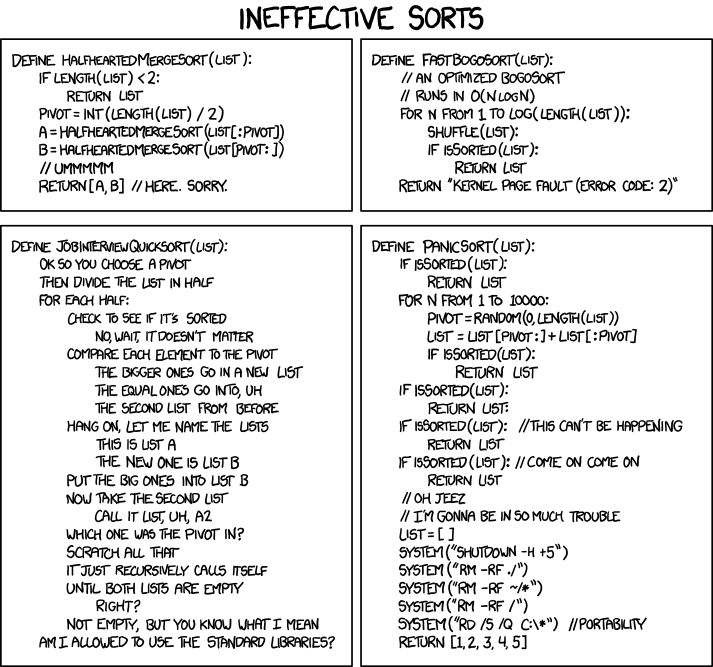
\includegraphics[width=0.8\textwidth]{ineffective_sorts}
\end{frame}


\end{document}